\documentclass[aspectratio=169]{beamer}

\usetheme{Madrid}
\usecolortheme{default}

\usepackage{graphicx}
\usepackage{amsmath}
\usepackage{booktabs}

\graphicspath{{../figures/}}

\title[Hybrid MC--Power PageRank]{Monte Carlo Methods in PageRank Computation:\\
When One Iteration Is Sufficient}
\subtitle{Hybrid Monte Carlo -- Power Iteration PageRank (Base Paper Review \& Implementation)}
\author{Afham Adian}
\date{\today}

\setbeamertemplate{navigation symbols}{}
\setbeamertemplate{footline}[frame number]

\begin{document}

% ---------------------------------------------------------------
\begin{frame}
  \titlepage
\end{frame}

% ---------------------------------------------------------------
\begin{frame}{Exact Solution: LU Decomposition}
  PageRank as a linear system:
  \[
    \bigl(I - d\,P^{\top}\bigr)\,\pi \;=\; \frac{1-d}{n}\,\mathbf{1}
  \]
  where $P$ is the (row-stochastic) transition matrix, $d$ the damping
  factor, and $\pi$ the unknown PageRank vector.

  \vspace{0.5cm}
  \textbf{LU approach:} factorize $A = I - dP^{\top} = LU$, then solve
  \[
    Ly = \frac{1-d}{n}\mathbf{1}, \qquad U\pi = y
  \]
  by forward/back substitution.

  \vspace{0.3cm}
  Exact, but $O(n^3)$ in general -- and sparse fill-in makes it
  impractical on large web graphs.
\end{frame}

% ---------------------------------------------------------------
\begin{frame}{Iterative Solution: Power Method}
  Google matrix:
  \[
    G \;=\; d\,P^{\top} + \frac{1-d}{n}\,\mathbf{1}\mathbf{1}^{\top}
  \]

  Power iteration:
  \[
    \pi^{(k+1)} \;=\; G\,\pi^{(k)}
  \]

  \vspace{0.4cm}
  At convergence, $\pi$ satisfies
  \[
    G\pi = \pi
  \]
  i.e.\ $\pi$ is the \textbf{eigenvector} of $G$ for eigenvalue $1$ --
  multiplying by $G$ no longer changes it, so the ranking has stabilized.
\end{frame}

% ---------------------------------------------------------------
\begin{frame}{Monte Carlo Techniques (5 Variants)}
  \small
  \begin{enumerate}
    \item \textbf{End-Point, Random Start} -- random start page, record only
      where each walk ends.
    \item \textbf{End-Point, Cyclic Start} -- start from every page in turn,
      record only the endpoint.
    \item \textbf{Complete Path, Cyclic Start} -- cyclic start, count every
      page visited along the walk.
    \item \textbf{Complete Path, Dangling Stop} -- cyclic start, count every
      visited page, walk stops at dangling nodes (no teleport).
    \item \textbf{Complete Path, Random Start} -- dangling-stop walk, but
      random starting page.
  \end{enumerate}
  \vspace{0.3cm}
  Common idea: simulate the random surfer thousands of times and count
  visits/endpoints instead of solving the system exactly.
\end{frame}

% ---------------------------------------------------------------
\begin{frame}{Our Hybrid Approach}
  \begin{itemize}
    \item \alert{MC warm start} (Complete Path, Dangling Stop) $\rightarrow$ quick rough estimate
    \item Seed \alert{Power Iteration} with it, instead of uniform $\tfrac{1}{n}\mathbf{1}$
    \item Result: \alert{fewer iterations}, same exact accuracy
  \end{itemize}

  \vspace{0.6cm}
  \centering
  \textbf{Monte Carlo (fast)} $\;+\;$ \textbf{Power Iteration (exact)} $\;=\;$ \textbf{Hybrid (fast \& exact)}
\end{frame}

% ---------------------------------------------------------------
\begin{frame}{Results: Relative Error at Ranks 1 / 10}
  \centering
  \begin{columns}[T,onlytextwidth]
    \column{0.5\textwidth}
      \centering
      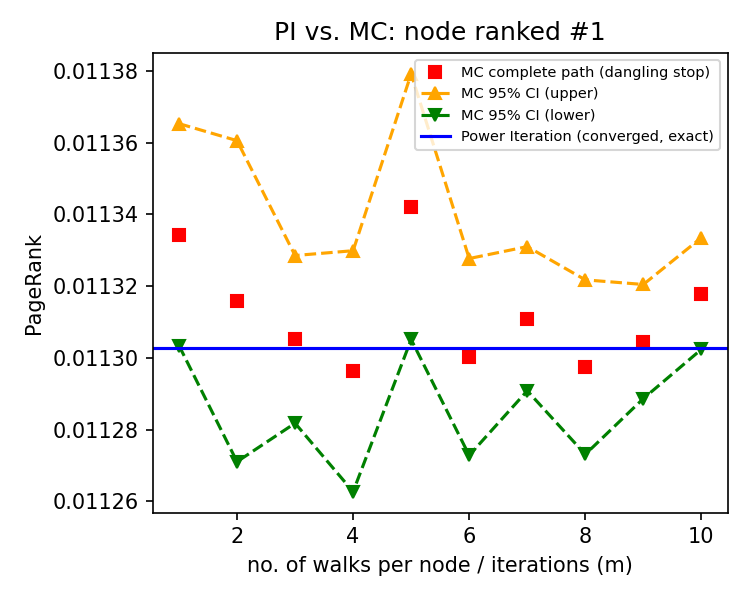
\includegraphics[width=\linewidth]{pi_1.png}\\
      \small Rank 1
    \column{0.5\textwidth}
      \centering
      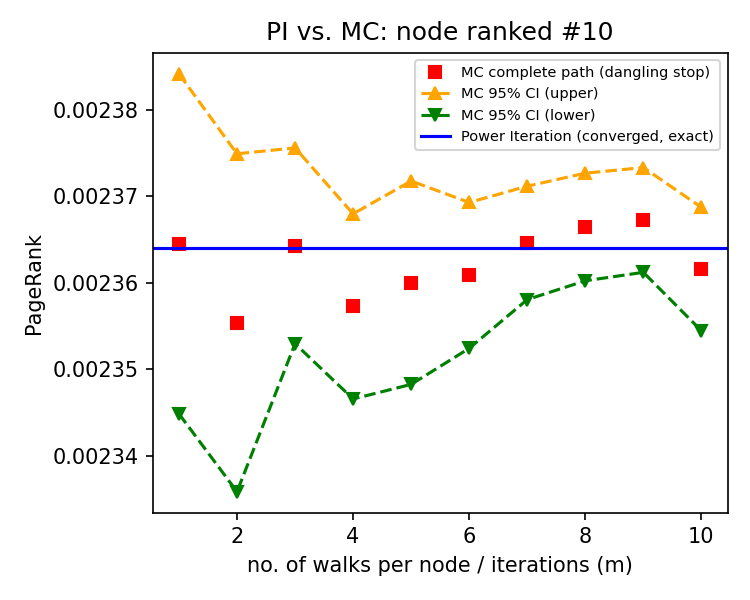
\includegraphics[width=\linewidth]{pi_10.png}\\
      \small Rank 10
  \end{columns}
\end{frame}

% ---------------------------------------------------------------
\begin{frame}{Results: Relative Error at Ranks 100 / 1000}
  \centering
  \begin{columns}[T,onlytextwidth]
    \column{0.5\textwidth}
      \centering
      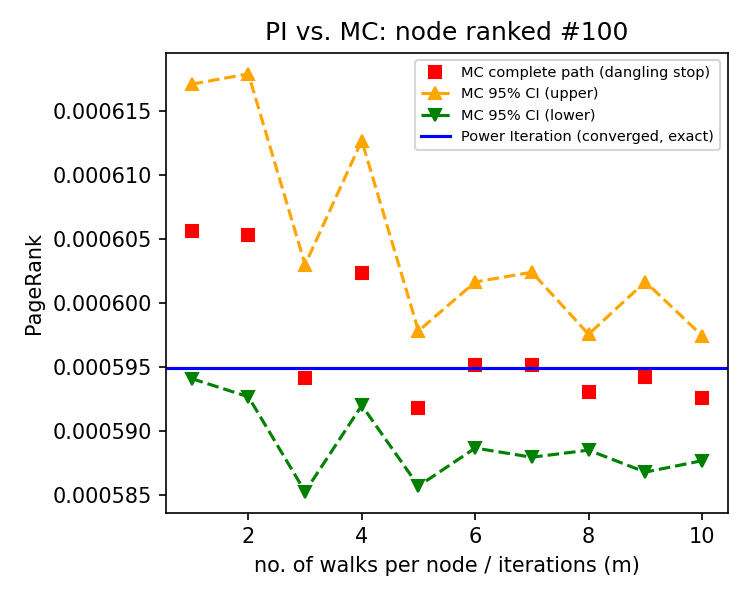
\includegraphics[width=\linewidth]{pi_100.png}\\
      \small Rank 100
    \column{0.5\textwidth}
      \centering
      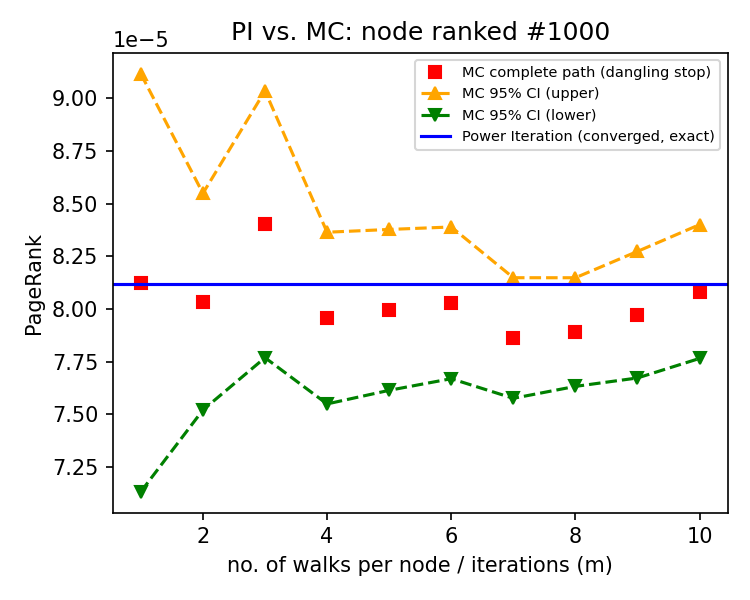
\includegraphics[width=\linewidth]{pi_1000.png}\\
      \small Rank 1000
  \end{columns}
\end{frame}

% ---------------------------------------------------------------
\begin{frame}{Results: Accuracy vs. Computational Cost}
  \centering
  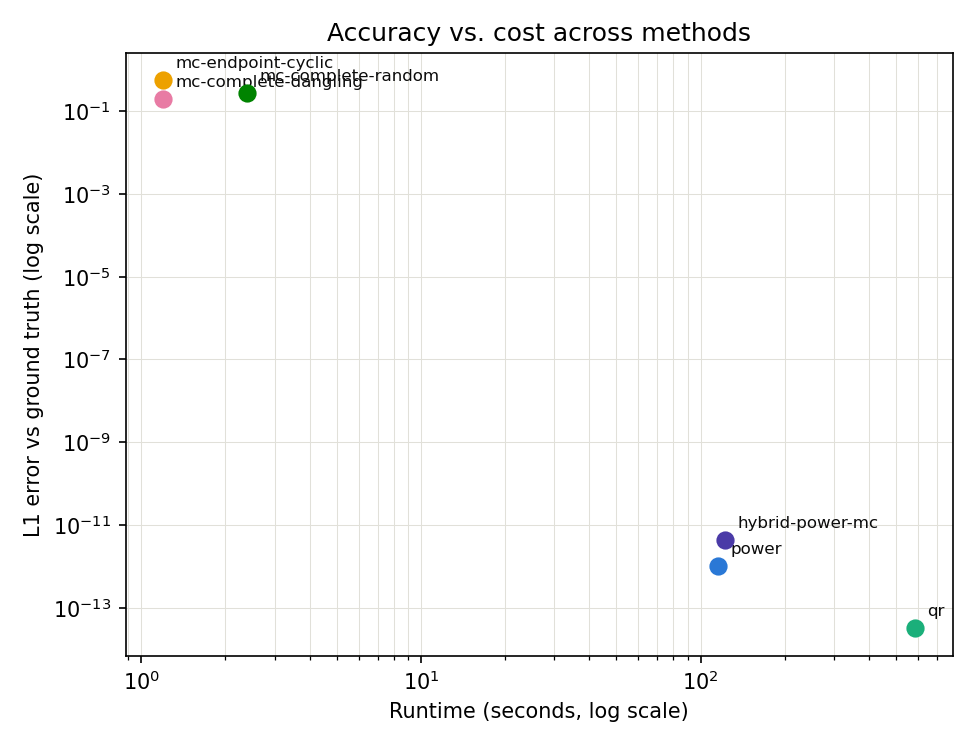
\includegraphics[width=0.75\linewidth]{accuracy_vs_cost.png}
\end{frame}

% ---------------------------------------------------------------
\begin{frame}{Results: Accuracy and Speed Comparison}
  \centering
  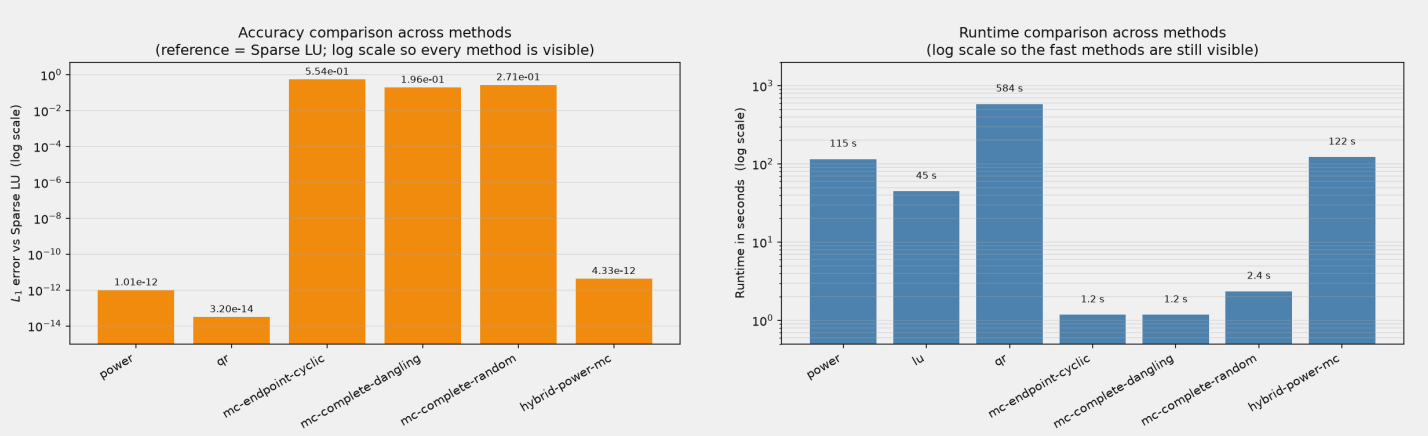
\includegraphics[width=0.95\linewidth]{acc_comp_log.png}
  \vspace{0.4cm}
  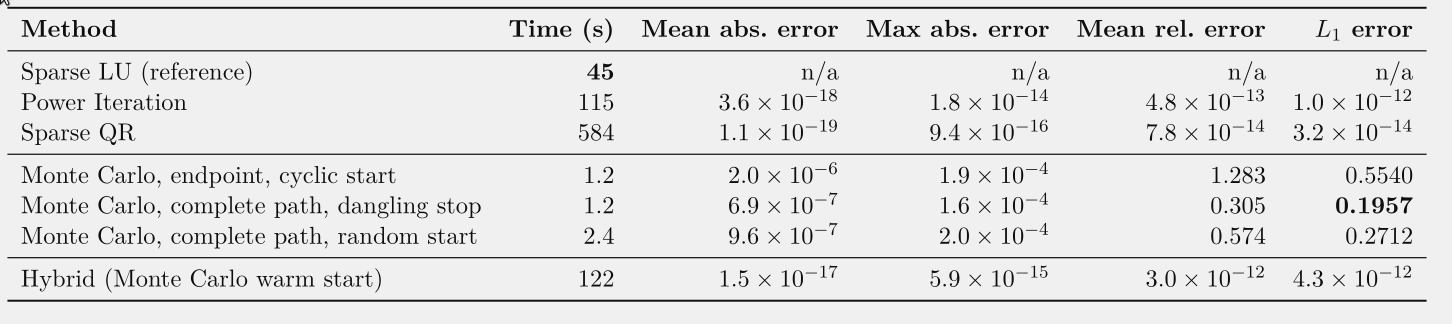
\includegraphics[width=0.95\linewidth]{speed_vs_accuraccy.png}
\end{frame}

% ---------------------------------------------------------------
\begin{frame}{Results: Hybrid vs. Power Iteration}
  \centering
  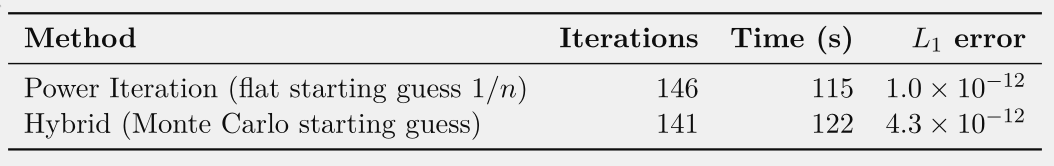
\includegraphics[width=\linewidth]{Hybrid_vs_power.png}

  \vspace{0.5cm}
  \begin{itemize}
    \item Warm start from MC estimate reduces the number of power-iteration
      steps needed to converge.
    \item Same exact final accuracy as cold-start power iteration, at lower
      total cost.
  \end{itemize}
\end{frame}

\end{document}
